\documentclass{article}
\usepackage[utf8]{inputenc}
\usepackage{graphicx}


\title{Relazione Operazionale}
\author{Francesco Pio Merafina, Onofrio Davide Caputo, Alessandro Lamesta}


\begin{document}

\maketitle

\section{Abstract:}
Nella presente relazione si illustra l’utilizzo di un amplificatore operazionale
come integratore di un segnale di tensione alternata in ingresso e si fornisce una
spiegazione delle procedure adottate allo scopo di affinare le misure.
~
\section{Cenni teorici:}
L'amplificatore operazionale consiste in una cascata di amplificatori differenziali, inoltre sappiamo che la componente ha un'alta resistenza di ingresso, una piccola resistenza in uscita, ed un grande valore di amplificazione. Per i nostri scopi tratteremo la componente come una scatola chiusa. Grazie alla modelizzazione fatta mediante il teorema di Miller, sappiamo che idealmente la funzione di trasferimento dipende dal rapporto tra l'impedenza in parallelo all'amplificatore e da quella in ingresso. Nel nostro caso l'impedenza in parallelo sarà un condensatore, il quale ha un comprtamento da integratore che viene fuori risolvendo il circuito.
~
\begin{figure}[h!]
    \centering
    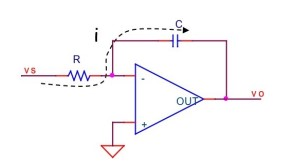
\includegraphics[width=\linewidth]{operazionale.jpg} 
    \caption{Schema di riferimento per l'esperiment}
    \label{figura1}
\end{figure}
~
\section{Strumentazione:}
La strumentazione usata per l'esperimento è la seguente:
\begin{itemize}
    \item generatore di forme 
    \item generatore di tensione continua
    \item condensatore da 68nF
    \item 1 resistore da 220kΩ
    \item 2 potenziometri da 10kΩ
    \item 1 amplificatore operazionale LM741
    \item oscilloscopio
    \item multimetro digitale
\end{itemize}
il tutto è stato montato su breadboard.
~
\section{Metodologia sperimentale:}
Sappiamo che il modello usato da noi come riferimento è di tipo ideale, quindi nella realtà dei fatta dobbiamo considerare alcuni effetti non previsti teoricamente. L'effetto più importante è quello della tensione di offset, questa tensione è dovuta al fatto che ci sono delle leggere asimmetrie all'interno dell'amplificatore, quindi per poter bilanciare questa tensione e fare in modo che non venga amplificata prima di tutto si è inserito un potenziometro tra due ingressi appositi previsti dal costruttore e lo regoliamo fino a bilancaire il circuito, ed inoltre per abbattere il guadagno di questa tensione inseriremo in parallelo al condensatore una resistenza.
~
\begin{figure}[h!]
    \centering
    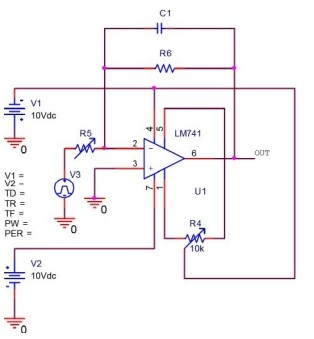
\includegraphics[width=\linewidth]{op1.jpg} 
    \caption{Schema del circuito effettivo utilizzato}
    \label{figura1}
\end{figure}
~
In ingresso si invia un segnale di onda quadra di ampiezza picco-picco 2V ad una frequenza di 1kHz, sapendo che come output vogliamo un'onda quadra dobbiamo ottenere che il periodo dell'onda quadra sia: $\tau$=0.25ms, e per ottenere questo, sapendo che la funzione di trasferimento dipende dalla resistenza in ingresso, variando il valore del potenziometro si è ottenuto un valore di resistenza di:3.80K$\Omega$, mentre la resistenza in parallelo ha un valore compres tra la 50 volte e 100 volte quella di ingresso.
~
\section{Appendice:}
Testi di riferimento:
\begin{itemize}
    \item Sedra, Smith, Microelectronic circuits, 5th ed. Oxford University Press,
2004
    \item Dell’Orso, Falchini, Flaminio et al. Introduzione all’elettronica digitale,
parte 2, Edizioni ETS, 2005

\end{itemize}
\end{document}